\documentclass[12pt,a4paper]{article} %scrbook}%bookof}



% makes nice font


%fills A4 page
\usepackage{a4wide}
\usepackage[inner=2cm,outer=2cm, bottom = 2.0cm]{geometry}   %nice setting for twoside binding



%\usepackage[utf8]{inputenc}   % damit man Umlaute direkt eingeben kann und diese erkannt werden.
\usepackage[T1]{fontenc}        % Umlaute werden als eine Einheit angesehen -> richtige Trennung;
% ausserdem: die T1-Fonts gibt es auch in
% größeren Größen
%\usepackage{ae,aecompl}
\usepackage{units}
\usepackage[english]{babel}      %hiermit erhält man z.B. 'Abb.' statt 'Fig.' bei Bildbeschriftungen
\usepackage[utf8]{inputenc}
%\makeglossary                   % zwischendurch makeindex disseration aufrufen
\usepackage{enumerate}
\usepackage{latexsym}


%\clearscrplain
%\clearscrheadings

\usepackage[headsepline]{scrlayer-scrpage}
%\usepackage[]{scrpage2}
%\clearplainofpairofpagestyles
%\clearscrheadings
\pagestyle{scrheadings}

\cofoot[\pagemark]{\pagemark}% optionales Argument --> plain
%\clearscrheadings
\rohead{NAWI Graz}
\chead{
	Exercise Statistical Physics \\{\small Contact: gerhard.dorn@tugraz.at}}
\lohead{ITP}
\usepackage{titlesec}
\titleformat{\section}
{\normalfont\large\bfseries}{\thesection}{1em}{}


\usepackage{amsmath,amsthm,amsfonts}
%\usepackage{showkeys}
%\usepackage{epsfig}
%\usepackage{epic}
\usepackage{xr}

\usepackage{graphicx}
%\usepackage{inmthesis}
\usepackage{hyperref}
\usepackage{verbatim}
\usepackage{tikz}
\usepackage[sorting=none, hyperref=true, backref=true]{biblatex}
\addbibresource{./library.bib}
%boxes
\usepackage{mdframed}
\usepackage{tensor}
%unity operator
%\usepackage{bbold}
 \setcounter{section}{9}
\begin{document}

 %\begin{center}
 %Technische Universität Graz \\
 %Institut für Theoretische Physik - computational physics \\
 %Prof. Dr. Wolfgang von der Linden \\
 %Kontakt: gerhard.dorn@tugraz.at
 %\end{center}
 
 
 \vspace{1cm}
 
 \section{ Negative Temperature}

Consider an isolated paramagnet consisting of $N$ spins of quantum number
$S = 1/2$ with an applied field $h$ along the $z$-direction. Considering the quantum numbers of the Pauli spin matrices $\sigma_l= \pm1$, the Hamiltonian is given by:

\begin{equation}
H= -h \sum_l \sigma_l
\end{equation}

The magnetization per lattice site is defined by $m = \langle \sigma \rangle$ and is independent of the lattice position $l$.

\begin{itemize}
 \item Calculate the entropy of the system as a function of magnetization.\footnote{You may ask the following questions: How many states are there for a fixed magnetization? How do you link the magnetization to the total number of positive spins $N_+$ .
 You will need Stirling's formula: $\ln N! \approx N \ln N - N$}
 \item Calculate the energy of the system as a function of magnetization.
 \item Derive a relation for temperature and plot the temperature as function of magnetization $T(m)$.
 \item How can the temperature become negative based on this relation?
 \item Is negative temperature a phyiscal quantity or what is implied by this negative value about the state of the system, regarding the equilibrium condition?
 
 \end{itemize}
 
 
\section{Engineering of copolymers}

Imagine a copolymere consisting of two different types of monomers, the radical parts, type $A$ (open brackets) and the passive parts, antioxidants, type $B$ (closed brackets).
The construction rule is the following: For each monomer of type $A$ another monomer (type $A$ or $B$) can attach. If there are as many monomers of type $A$ and $B$ only radicals can attach. (Think of the valid bracket sequences of the first assignment). 
We will work with two variables, the total length of the monomer $N = |A|+|B|$ and the fraction of radicals $x = \frac{|A|}{N}$.
\begin{itemize}
 \item What is the allowed range of $x$?
\end{itemize}

\paragraph{Microcanonical picture}
\begin{itemize}
 \item What is the total number of polymers $Z(x,N)$ of length $N$ (total number of monomers) with $N\cdot x$ radicals (monomers of type $A$).\\
Hint: Recall the bracket counting problem of the first assignment (Problem~1) and reformulate the result to express the number in terms of $x$ and $N$.
\item What is the associated entropy $S(x,N)$? Use the Stirling formula to resolve the factorials.\\
What do you have to do in order to guarantee extensivity of the entropy?
\item After having done this approximation (it's easier in the logarithm) derive the following approximate expression for the partition sum: $$Z(N,x) \approx  \left(\frac{1}{x^x (1-x)^{1-x}}\right)^N \underbrace{\left(1 - \frac{1-x}{x+\frac{1}{N}}\right)}_{\approx 1 \,(\mathcal{O}(1))}$$
\end{itemize}

Each possible polymer configuration is linked with an energy term which is dependent on the total number of monomers $N$ and the fraction of radicals $x$. Each monomer (type $A$ or type $B$) costs an energy $\varepsilon$ (increases the energy), each monomer of type $A$ (radical) lowers the energy by $\Delta$ whereas each monomer of type $B$ increases the energy by $\Delta$. 
\begin{itemize}
 \item State the described formula for energy depending on the total number of monomers $N$ and on the ratio of radicals $x$: $E(x,N)$.
\end{itemize}


%\begin{align}
% E(N,M) = N \varepsilon - (2M-N) \Delta
%\end{align}
It will be now our aim to predict the average radical fraction $\langle x \rangle$ in our polymers depending on the temperature $T$. 

\paragraph{Canonical ensemble}
Now we look at the polymerization in a heat bath, the total number of particles $N$ shall remain fixed (this corresponds to a fixed density of monomers in the polimerization process).

There are two paths to reach our goal which are depicted in Fig.~\ref{fig:paths}. Going the tough one will bring you an extra point.

\begin{figure}
 \begin{center}
  \begin{tikzpicture}
  \node (A) at (-0.5,0) {$Z^\textnormal{micro}(x,N)$};
  \node (B) at (3,0) {$S(x,N)$};
  \node (C) at (6.5,0) {$S(E,N)$};
  \node (D) at (10,0) {$E(T,N)$};
  \node (E) at (4.75, -1.5) [draw] {$E(x,N) = a\cdot N + b\cdot x$};
  \node (F) at (4.75, -0.75) [anchor = east] {$x(E,N)$};
  \node (G) at (8.25, 1.5) [draw] {$\frac{\partial S}{\partial E} \overset{!}{=} \frac{1}{T}$};
  \node (H) at (10, -1.5) [draw] {$E(T,N) = a\cdot N + b\cdot \langle x \rangle$};
  %as
  \draw[->] (node cs:name=A) -- (node cs:name=B);
  \draw[->] (node cs:name=B) -- (node cs:name=C);
  \draw[->] (node cs:name=C) -- (node cs:name=D);
  \draw[->] (node cs:name=D) -- (10,-1);

  \draw[->] (node cs:name=E) -- (4.75,-0.2);
  \draw[->] (node cs:name=G) -- (8.25,+0.2);
  
  \node (I) at (1.9, -3.5) {$Z^\textnormal{can}(T,N) = \int e^{-\beta E(x,N)} Z^\textnormal{micro}(x,N) dx$};
  \node (J) at (2.45, -4.5) {\footnotesize Saddle point approximation};
  \node (K) at (1, -5.5) {{\footnotesize get} $p(x)$};
  \node (L) at (-0.5, -6.5) {$\langle x \rangle = \int x p(x) dx$};
  
  \node (M) at (1, -2.5) [red] {\footnotesize hard way};
  
  \draw[->, red] (node cs:name=A) -- (-0.5, -3);
  \draw[->, red]  (-0.5, -4) -- (node cs:name=L);

  
  \end{tikzpicture}
\caption{Sketch of the two ways to derive at the average ratio of radicals in the copolymer.}
 \end{center}
\label{fig:paths}
\end{figure}


The easy way uses a trick by introducing the temperatur via the energy which has the form $E(x,N) = ax+bN$.
Expressing $x(E,N)$ and plugging this into the entropy allows us to do the derivation with respect to the energy and define the temperature as $$\frac{1}{T} = \frac{\partial S(E,N)}{\partial E}.$$ 
This relation can be used to express $E(T,N)$ and comparing this expression with $E(x,N)$ allows us to identify $\langle x \rangle$. 

\begin{itemize}
 \item Calculate the internal energy depending on the temperature and derive the average ratio of radicals in the polymer $\langle x \rangle$
 \item Which parameters ($N$, $T$, $\varepsilon$, $\Delta$) have an influence on the ratio of radicals?\\
 Sketch  $\langle x \rangle$ as function of $T$ (the other parameters shall have fixed positive values).
 \item Calculate the specific heat $c_V$. Is it in agreement with the laws of thermodynamics?
 \item Check if the third law of thermodynamics is fulfilled.
\end{itemize}


The tough way:
\begin{itemize}
 \item[+] Calculate the canonical partition function using the result from the microcanonical partition sum.
 \item[+] Approximate the sums by integrals and solve the integral analytically using the stationary point (saddle point) approximation and the error function. You should end with an analytic expression for $Z_{\textnormal{can}}(T,N)$. 
 \item[+] Derive the probability distribution for $p(x)$.
 \item[+] Calculate $\langle x(T,N)\rangle$.
\end{itemize}

\paragraph{Grandcanonical ensemble}
Now we allow an arbitrary growth and as such a variation of the length of the polymers $N$. 
\begin{itemize}
 \item Calculate the chemical potential $\mu$ and plot it as a funtion of temperature $T$ for fixed positive values of the other relevant parameters.
\end{itemize}



\section{Space catastrophe}

Assume to have a space ship with an interiour of 3 m$^3$ filled with air (ideal gas assumption) with a pressure of $P = 10^5$ Pa and a temperature of $270$ K. 
Due to space debris we find tiny holes in the hull of our spacespip (effusion condition fulfilled) with a total area of 10 cm$^2$. 

\begin{figure}
	\begin{center}
		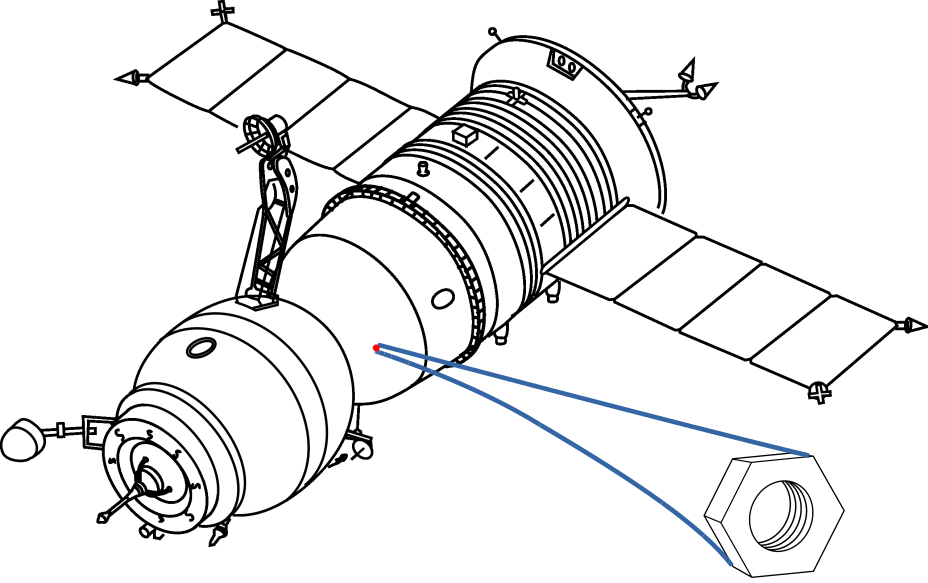
\includegraphics[width = 0.7\textwidth]{space_ship.png}
		\caption{Illustration of a nut (space debries) hitting a Soyus capsule.}
	\end{center}
\end{figure}
\paragraph{Mass spectrometer}
According to Graham's law the effusion is dependent on the mass of the outgoing particles.
\begin{itemize}
\item What is the gas distribution (related to the volume and related to mass) of air? 
\item What will be the average distribution outside the space ship due to effusion (related to volume and related to mass)?
 \item What is the average mass of one gas particle inside the spaceship?
 
 \end{itemize}
 \paragraph{Cooling of the spaceship}
 From the ideal gas equation (Joule expansion, free expansion, experiment of Gay-Lussac) we would not expect the temperature to change. 
 
 \begin{itemize}
 \item What is the average  energy of one particle inside the spaceship?
 \item What is the average  energy of one particle leaving the spaceship?
 \item How is the average energy of one particle related to the temperature inside the space ship?
 \item What will be the temperature outside of the spaceship?
 \item What is the average mean free path of the gas particles\footnote{You need to assume a diameter for the gas molecules.}? Draw a sketch depending on the number of particles.
\end{itemize}
Since particles with a higher average energy will leave the space ship the average energy per particle inside the space ship has to go down.\footnote{Look at the chapter effusion in the lecture notes.}
\begin{itemize}
 \item Derive a differential equation for the change of temperature inside the space ship and solve it.
 \item Sketch the pressure $p(t)$ and the temperature $T(t)$ over time.
\end{itemize}

\paragraph{[Bonus:] Human being as thermodynamic machine}
The human body has a power of approximately 100 W in the form of heat. We get rid of this heat by radiation to the environment and by convection (for simplistic reasons we neglect sweating).
The emission of heat via radiation is dependent on the temperature of the wall which as such also radiates back. 
\begin{itemize}
 \item Find the (a) differential equation describing the heat transfer $\frac{dQ_\textnormal{r}}{dt}$ via radiation depending on the temperature of the wall $T$ (we assume this temperature to be equal to the temperature of the air inside the space ship), the temperature of the human body $T_h = 37^\circ$ C, the area of the spaceship walls and the area of the human surface (skin).
\end{itemize}

The heat emission via convection is dependent on the temperature gradient and the pressure of the air.

\begin{itemize}
\item Derive a differential equation describing the heat transfer $\frac{dQ_\textnormal{c}}{dt}$ via convection depending on the temperature $T$ of the air, the pressure $p$ and the human body temperature $T_h$ (and the area of the human skin).
 \item Now combine everything and examine the change of heat transfer $\frac{d^2 Q}{dt^2}$ of radiation and convection due to the hole in the wall causing pressure drop and temperature drop in the differential equations. 
\item Is the heat emission increasing (the astronaut is getting colder) or decreasing (the astronaut is getting warmer)?
\end{itemize}




% \printbibliography



\vspace{2cm}
\begin{minipage}[t]{1\textwidth}
	\raggedleft
	\centering
	
\includegraphics[width = 0.20\textwidth]{CC-BY_icon}
	\vspace{0.2cm}
	
	\centering
	{\Large Gerhard Dorn} \\
	https://creativecommons.org/licenses/by/4.0/legalcode
\end{minipage}



  \end{document}
  
  
